\chapter{Loewner Evolutions of Anisotropic Systems}
\label{ch6-asle}

Lorem ipsum dolor sit amet, consectetur adipisicing elit, sed do eiusmod tempor
incididunt ut labore et dolore magna aliqua. Ut enim ad minim veniam, quis
nostrud exercitation ullamco laboris nisi ut aliquip ex ea commodo consequat.
Duis aute irure dolor in reprehenderit in voluptate velit esse cillum dolore eu
fugiat nulla pariatur. Excepteur sint occaecat cupidatat non proident, sunt in
culpa qui officia deserunt mollit anim id est laborum.

\section{Generating Fractional Browninan Motions}
\label{sec:fbm}

We want to generate fractional Brownian motions $B_t$ such that
\begin{equation}
    \label{eq:fbm}
    \left\langle B_t^2 \right\rangle = bt^{2H}.
\end{equation}
There are several methods to generate this process numerically, but not all of
them give you ample control over the prefactor $b$, although most are very
accurate in $H$. A method that adequately fulfills this criterion is the
Davies-Harte algorithm. It can be used to generate any stationary Gaussian
process for which the autocovariance sequence is known. In the case of
the fractional Brownian motion, it takes the form
\begin{equation}
    c_i = \frac{b}{2} \left(
            \left|i+1\right|^{2H} +
            \left|i-1\right|^{2H} -
            2\left|i\right|^{2H}
          \right)
\end{equation}

To obtain a series of length $N$ we generate the following sequence of $2N$
points
\begin{equation}
    s_i=\left\{c_{0},c_{1},\ldots,c_{N},c_{N-1},\ldots,c_{1}\right\}
\end{equation}
and compute its discrete Fourier transform, that is
\begin{equation}
    g_{i}=\sum_{j}s_{j}e^{-i\pi kj/N}.
\end{equation}
This operation can be done in $O(N\log N)$ operations using a fast Fourier
transform. The $g_i$ are real valued, but a necessary condition for the
Davies-Harte algorithm to work is that they also be nonnegative. It is
important to check for this condition even if just for debugging purposes,
as it catches a lot of small mistakes.

Let $W_{i\in[0,N]}$ be a sequence of $N+1$ random complex numbers where the
real and imaginary parts are independently distributed according to a normal
distribution with zero mean and unit variance. We then construct the series
\begin{equation}
    Y_{i\in[0,2N-1]}=\begin{cases}
        \sqrt{2Ng_{i}}\mbox{Re}\left\{ W_{i}\right\}  & \mbox{if } i=0,N\\
        \sqrt{Ng_{i}}W_{i} & \mbox{if } i\in\left[1, N-1\right]\\
        \sqrt{Ng_{i}}W_{2N-i}^{*} & \mbox{if } i\in\left[N+1, 2N-1\right]
    \end{cases},
\end{equation}
where $W^{*}$ is the complex conjugate. The fractional Brownian motion $B_t$ is
obtained by computing the inverse Fourier transform of this series. Although
the obtained series have $2N$ points we discard the second half, as it is not
guaranteed to be well behaved. The $B_t$ are defined for $t\in{0,1,\ldots,N-1}$,
but the series can easily be rescaled for any timespan desirable by applying
the relation
\begin{equation}
    B_{t\in[0,t_{f}]}={\left(\frac{t_{f}}{N}\right)}^{H}B_{t\in[0,N]}.
\end{equation}

In Figure~\ref{fig:fbm}, we show some examples of fractional Brownian motion
generated using this algorithm. We also show that the mean squared displacement
behaves as described by Eq.~\ref{eq:fbm}.

\begin{figure}
\begin{center}
    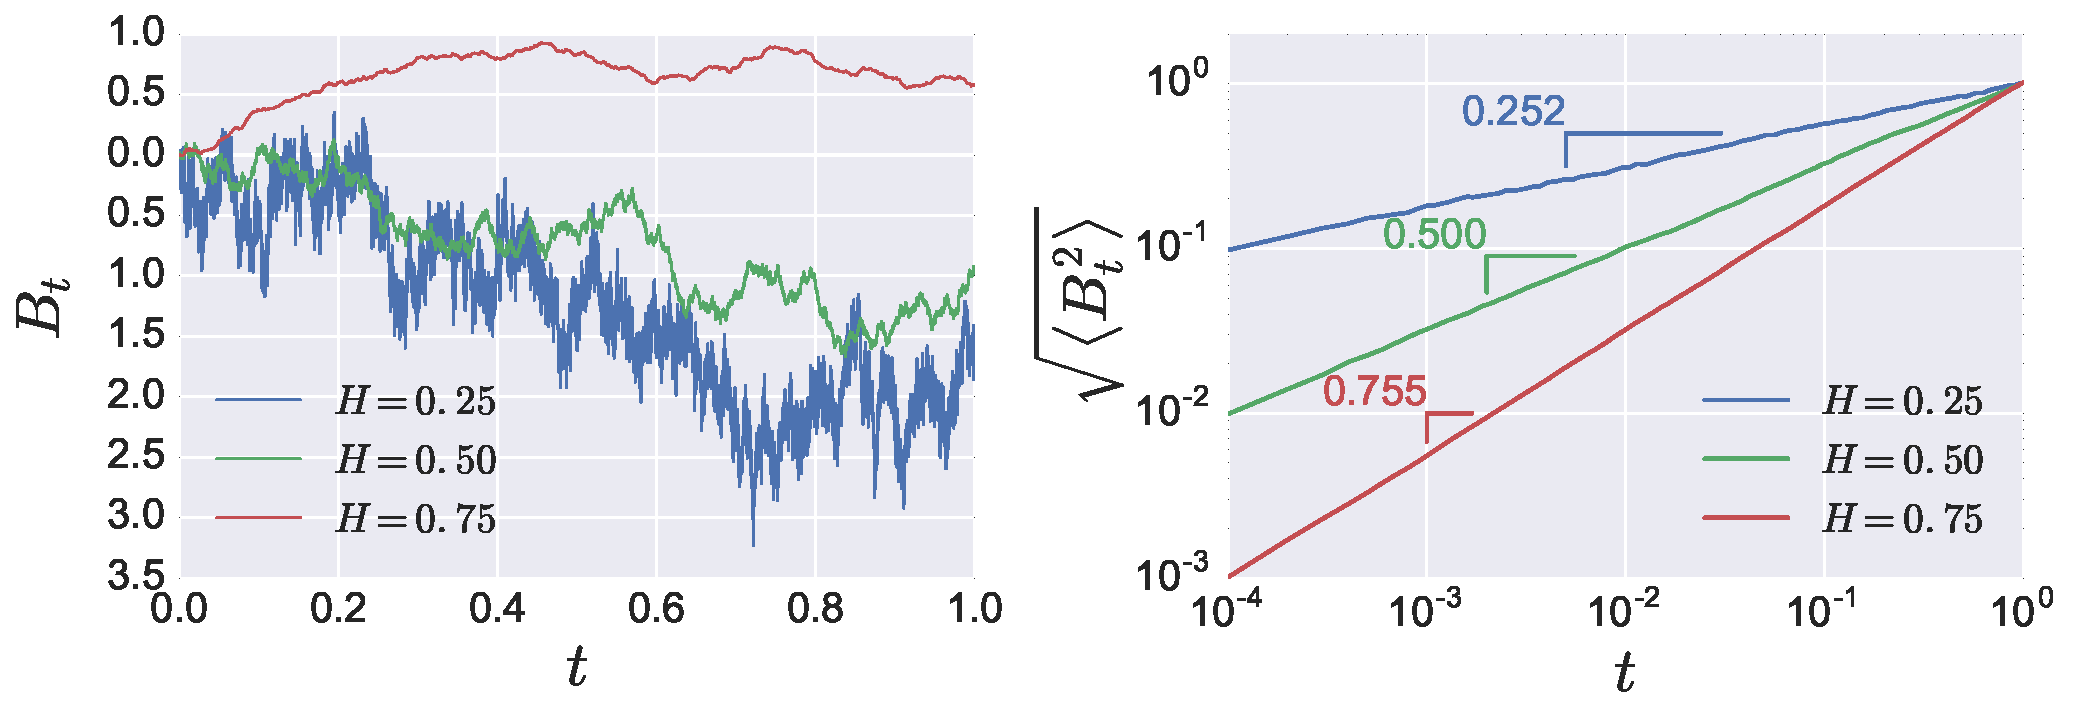
\includegraphics[scale=0.45]{chapters/ch6-asle/figs/fbm}
\end{center}
\caption{Example of three fractional Brownian motions generated using the
    Davies-Harte algorithm (left). They all have $b=1.0$ and different values
    of $H$. We also show the behavior of the mean square displacement of the
    scaling properties of the curves. We found that the mean square displacement
    scales as $\sqrt{\left\langle B_t^2\right\rangle}=\sqrt{b}t^H$ with
    parameters very similar to the input given.}
\label{fig:fbm}
\end{figure}
